\chapter{Réalisation et validation}
\label{chap:implementation}

\section*{Introduction}

Ce chapitre présente la traduction effective de la conception en une application
exécutable. Il ne décrit pas seulement les écrans obtenus : il relie les incréments
du Product Backlog aux composants frontend, aux services métier, aux données
persistées, aux processus d'infrastructure et aux contrôles qui permettent de
vérifier leur comportement.

La réalisation a été menée par incréments dépendants. Chaque incrément stabilise
une capacité démontrable avant d'ouvrir le suivant. Cette progression a d'abord
sécurisé l'identité et l'isolation des organisations, puis le référentiel des
stations, la communication OCPP, les opérations terrain, la recharge, le paiement
et enfin le pilotage commercial. Elle aboutit à un premier parcours vertical :

\begin{center}
\textbf{borne simulée $\rightarrow$ OCPP $\rightarrow$ disponibilité
$\rightarrow$ alerte ou carte $\rightarrow$ session $\rightarrow$ tarif
$\rightarrow$ paiement simulé $\rightarrow$ reçu.}
\end{center}

Les résultats présentés correspondent à l'état du dépôt au 28 juillet 2026. Une
fonctionnalité est qualifiée de \emph{réalisée} lorsqu'elle possède un contrat
backend, une interface exploitable et des tests automatisés adaptés. Le terme
\emph{validée localement} ne signifie pas qu'elle est déjà certifiée pour la
production : les limites relatives à une borne physique, à un prestataire de
paiement réel, au déploiement et à la charge sont indiquées explicitement.

\section{Environnement de développement}

\subsection{Outils et choix technologiques}

Le développement est effectué sur un poste Windows avec PHP installé localement
et Docker Desktop appuyé sur WSL2 pour les composants conteneurisés. Cette
organisation conserve un cycle rapide pour l'interface et l'API tout en isolant
la passerelle OCPP, le simulateur de bornes et le simulateur de paiement. Git
assure la traçabilité du code et GitHub centralise le dépôt distant.

\begin{table}[H]
  \centering
  \caption{Environnement technique effectivement utilisé}
  \label{tab:implementation-toolchain}
  \begin{tabularx}{\textwidth}{|p{3.2cm}|p{4.0cm}|Y|}
    \hline
    \rowcolor{ctmint}
    \textbf{Domaine} & \textbf{Technologies} & \textbf{Usage dans le projet}\\\hline
    Frontend & React 19, TypeScript 6, Vite 8 &
    Application monopage, typage statique et compilation.\\\hline
    Interface & Ant Design 6, Recharts, Leaflet, GSAP &
    Composants, graphiques, cartes et animations ciblées.\\\hline
    État et échanges & TanStack Query, Axios, Zustand &
    Cache serveur, appels HTTP et états locaux transverses.\\\hline
    Backend & PHP 8.5, Laravel 13 &
    API REST, logique métier, validation, autorisation et tâches planifiées.\\\hline
    Identité & Sanctum, Socialite, Spatie Permission &
    Session SPA, Google OAuth 2.0, rôles et permissions.\\\hline
    Données & PostgreSQL 16, Eloquent &
    Persistance transactionnelle, relations et migrations.\\\hline
    Temps réel & Reverb, Laravel Echo &
    Notifications et mises à jour poussées par WebSocket.\\\hline
    OCPP & Python 3.11, OCPP 1.6J, simulateur SAP &
    Passerelle WebSocket, messages de borne et scénarios de test.\\\hline
    Paiement & Contrat \texttt{PaymentGateway}, WireMock 3 &
    Fournisseur externe simulé, webhooks et scénarios d'erreur.\\\hline
    Email & Resend, queue Laravel &
    Vérification d'email, invitations et notifications asynchrones.\\\hline
    Qualité & PHPUnit 12, Oxlint, TypeScript &
    Tests backend, analyse frontend et validation de compilation.\\\hline
    Documentation & \LaTeX, TikZ, OpenAPI 3.1 avec Scramble &
    Rapport, schémas et spécification versionnée de l'API.\\\hline
  \end{tabularx}
\end{table}

Les dépendances sont verrouillées par \texttt{composer.lock} et
\texttt{pnpm-lock.yaml}. Les valeurs sensibles sont placées dans les fichiers
\texttt{.env}, exclus de Git. Les fichiers \texttt{.env.example} documentent
uniquement les variables attendues, sans contenir de secret.

\subsection{Langages de programmation utilisés}

\begin{table}[H]
  \centering
  \caption{Langages utilisés dans la réalisation}
  \label{tab:implementation-languages}
  \begin{tabularx}{\textwidth}{|p{3.2cm}|p{3.8cm}|Y|}
    \hline
    \rowcolor{ctmint}
    \textbf{Langage} & \textbf{Composant} & \textbf{Responsabilité}\\\hline
    PHP & Backend Laravel &
    API REST, services métier, jobs, policies et tests.\\\hline
    TypeScript / TSX & Frontend React &
    Pages, composants, contrats API et interactions utilisateur.\\\hline
    Python & Passerelle OCPP &
    WebSocket OCPP, adaptation des messages et tests du protocole.\\\hline
    SQL & PostgreSQL &
    Migrations, contraintes, index et requêtes d'agrégation.\\\hline
  \end{tabularx}
\end{table}

\subsection{Organisation du dépôt et environnement d'exécution}

Le dépôt sépare physiquement les composants tout en proposant des commandes
communes à sa racine :

\begin{description}[leftmargin=37mm,style=nextline]
  \item[\texttt{frontend/}] application React et ressources visuelles ;
  \item[\texttt{backend/}] API Laravel, services, migrations, policies et tests ;
  \item[\texttt{ocpp-gateway/}] passerelle Python entre les bornes et Laravel ;
  \item[\texttt{infra/ocpp/}] composition Docker et profils du simulateur SAP ;
  \item[\texttt{infra/payment-simulator/}] serveur WireMock et contrats simulés ;
  \item[\texttt{scripts/}] commandes d'orchestration et de pilotage ;
  \item[\texttt{docs/}] rapport, API, manuels et cahier de tests.
\end{description}

\begin{figure}[H]
  \centering
  \resizebox{0.94\textwidth}{!}{\begin{tikzpicture}[
  font=\sffamily\small,
  process/.style={
    draw=ctline, rounded corners=2mm, thick, fill=white,
    minimum width=34mm, minimum height=13mm, align=center
  },
  hostproc/.style={process, draw=ctgreen, fill=ctmint},
  container/.style={process, draw=ctblue, fill=blue!5},
  optional/.style={process, dashed, draw=ctgray, fill=gray!4},
  flow/.style={{Latex[length=2.2mm]}-{Latex[length=2.2mm]}, thick, draw=ctgray},
  zone/.style={draw=ctline, rounded corners=3mm, dashed, inner sep=6mm}
]
  \node[hostproc] (vite) at (0,2.2) {Vite\\\texttt{:5173}};
  \node[hostproc] (laravel) at (5.0,2.2) {Laravel API\\\texttt{:8000}};
  \node[hostproc] (reverb) at (10.0,2.2) {Reverb\\\texttt{:8080}};
  \node[hostproc] (worker) at (2.5,-0.1) {Queue worker};
  \node[hostproc] (scheduler) at (7.5,-0.1) {Scheduler};

  \node[container] (postgres) at (0,-4.2) {PostgreSQL\\\texttt{:5432}};
  \node[optional] (mailpit) at (5.0,-4.2) {Mailpit optionnel\\\texttt{:8025/1025}};
  \node[container] (wiremock) at (10.0,-4.2) {WireMock\\\texttt{:9090}};
  \node[container] (gateway) at (0,-6.8) {Gateway OCPP\\\texttt{:9000}};
  \node[container] (sap) at (5.0,-6.8) {Simulateur SAP\\\texttt{:8082}};

  \draw[flow] (vite) -- (laravel);
  \draw[flow] (vite) to[bend left=18] (reverb);
  \draw[flow] (laravel) -- (reverb);
  \draw[flow] (laravel) -- (worker);
  \draw[flow] (laravel) -- (scheduler);
  \draw[flow] (laravel.south) to[out=-115,in=75] (postgres.north);
  \draw[dashed, flow] (worker.south) to[out=-35,in=160] (mailpit.west);
  \draw[flow] (laravel.south) to[out=-145,in=70] (gateway.north);
  \draw[flow] (gateway) -- (sap);
  \draw[flow] (laravel.south east) to[out=-35,in=95] (wiremock.north);

  \node[zone, fit=(vite)(laravel)(reverb)(worker)(scheduler),
    label={[ctgreen]above:\textbf{Processus hôte}}] {};
  \node[zone, fit=(postgres)(mailpit)(gateway)(sap)(wiremock),
    label={[ctblue]above:\textbf{Docker Desktop / WSL2}}] {};
\end{tikzpicture}
}
  \caption{Architecture de déploiement de l'environnement local}
  \label{fig:deployment-architecture}
\end{figure}

En production, les fichiers frontend doivent être servis derrière HTTPS,
l'application PHP doit être supervisée et les connexions OCPP doivent utiliser
\texttt{wss://}. Les workers, le scheduler, Reverb et la passerelle OCPP
constituent des processus distincts à superviser.

\subsection{Processus de développement}

Le fichier \texttt{package.json} racine sert de façade aux commandes des
différents environnements :

\begin{table}[H]
  \centering
  \caption{Commandes principales de l'environnement local}
  \label{tab:implementation-commands}
  \begin{tabularx}{\textwidth}{|p{4.4cm}|Y|}
    \hline
    \rowcolor{ctmint}
    \textbf{Commande} & \textbf{Responsabilité}\\\hline
    \texttt{pnpm dev:frontend} & Lance Vite sur le port 5173.\\\hline
    \texttt{pnpm dev:backend} & Lance l'API Laravel sur le port 8000.\\\hline
    \texttt{pnpm dev:queue} & Traite les emails et travaux asynchrones.\\\hline
    \texttt{pnpm dev:scheduler} & Exécute les règles périodiques.\\\hline
    \texttt{pnpm dev:reverb} & Lance le serveur WebSocket applicatif.\\\hline
    \texttt{pnpm ocpp:up} & Démarre la passerelle et le simulateur OCPP.\\\hline
    \texttt{pnpm ocpp:plug} / \texttt{ocpp:unplug} &
    Simule la connexion ou le retrait physique d'un câble.\\\hline
    \texttt{pnpm payment:up} & Démarre le fournisseur WireMock.\\\hline
    \texttt{pnpm build:frontend} & Vérifie les types et compile le frontend.\\\hline
    \texttt{pnpm test:backend} & Exécute la campagne PHPUnit.\\\hline
  \end{tabularx}
\end{table}

Le scheduler recalcule périodiquement la disponibilité, expire les commandes
OCPP, contrôle les SLA et génère les maintenances récurrentes. L'option
\texttt{withoutOverlapping} empêche le chevauchement d'une même tâche.

Chaque bloc fonctionnel est suivi d'un commit cohérent puis poussé sur la branche
\texttt{main}. Cette discipline facilite l'identification d'une régression. Les
fichiers d'environnement, les dépendances installées et les sorties temporaires
ne sont pas versionnés.

\section{Réalisation des fondations techniques}

\subsection{INC-01 : entrée, identité et multi-tenant}

\subsubsection{Parcours d'entrée}

L'entrée dans \ProjectName{} dépend du type d'utilisateur. Un client peut créer
son propre compte local, vérifier son adresse email, définir son mot de passe ou
continuer avec Google. Un employé ne s'inscrit pas librement : l'administrateur de
son organisation crée le compte opérateur ou technicien, puis une invitation
temporaire permet au destinataire d'activer son accès et de choisir son mot de
passe. Enfin, un futur administrateur commence par une demande de démonstration.
Le super administrateur étudie la demande, crée l'organisation et émet
l'invitation de l'administrateur.

Cette séparation résout deux problèmes métier. Premièrement, un compte employé ne
peut pas s'attribuer lui-même une organisation ou un rôle privilégié.
Deuxièmement, une demande de démonstration ne crée aucune ressource sensible avant
la décision du super administrateur. Les invitations sont révocables, renouvelables
et limitées dans le temps.

Le backend s'appuie sur Sanctum pour la session de la SPA et sur Socialite pour
Google OAuth. Le service \texttt{GoogleAccountService} associe l'identité externe
à un compte local sans importer les rôles Google. L'API locale reste propriétaire
du rôle, des permissions, de l'organisation et de l'état du compte. Les formulaires
d'inscription, de connexion, d'activation et de demande de démonstration possèdent
des règles de limitation et des réponses d'erreur structurées.

\subsubsection{Isolation organisationnelle}

Les administrateurs, opérateurs et techniciens appartiennent à une seule
organisation. Un client reste indépendant et peut utiliser les stations ou
souscrire aux plans de plusieurs organisations. Cette asymétrie est conservée
dans le modèle de données : l'appartenance d'un employé détermine son périmètre,
alors que les relations d'un client avec les organisations sont dérivées de ses
abonnements et de ses sessions.

La protection ne repose pas sur le menu React. Le middleware
\path{EnsureUserOrganizationScope}, les policies et les requêtes Eloquent
filtrent le périmètre côté serveur. Par exemple, un administrateur peut gérer les
employés et consulter les clients de son organisation, mais il ne peut pas
modifier un utilisateur d'une autre organisation en changeant simplement un
identifiant dans l'URL. Les tests d'API couvrent ces refus d'accès.

\subsubsection{Onboarding orienté vers la première valeur}

Après sa première connexion, chaque rôle reçoit un parcours court qui confirme son
contexte puis propose une première action utile. L'administrateur prépare
l'identité de son organisation, invite un employé puis enregistre une station.
L'opérateur rejoint directement la supervision, le technicien consulte son
travail assigné et le client recherche une station. Le parcours peut être quitté
et repris ; il ne bloque pas l'application.

\begin{figure}[H]
  \centering
  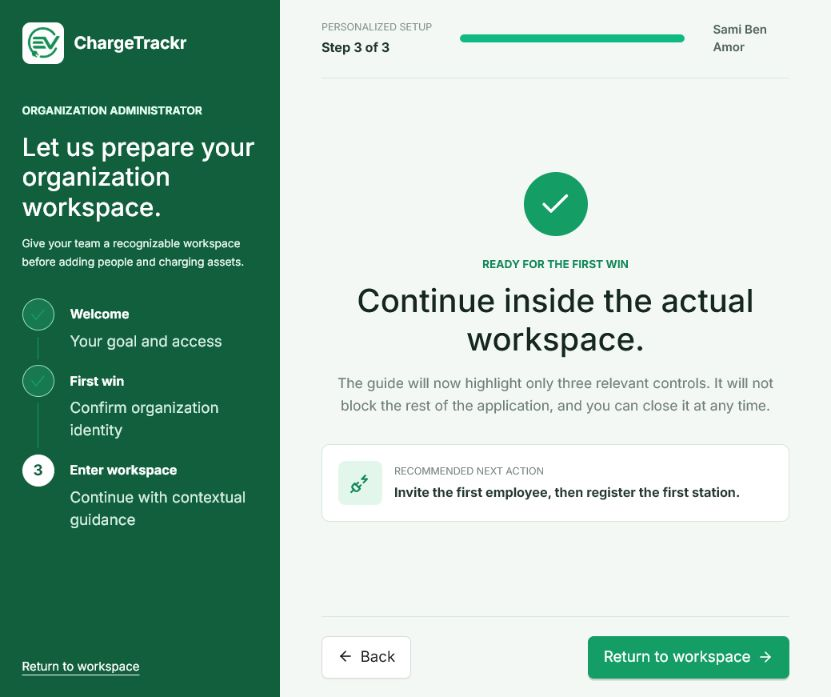
\includegraphics[width=0.92\textwidth]{assets/screenshots/onboarding-welcome.png}
  \caption{Dernière étape de l'onboarding de l'administrateur}
  \label{fig:implementation-onboarding}
\end{figure}

Les classes \path{AccountInvitationService} et
\path{DemoProvisioningService}, les contrôleurs d'authentification et les
policies concrétisent l'incrément. Les campagnes
\path{AuthApiTest}, \path{GoogleOAuthTest},
\path{DemoRequestWorkflowTest}, \path{OnboardingApiTest},
\path{OrganizationManagementApiTest} et
\path{UserManagementApiTest} fournissent la preuve automatisée principale.

\subsection{INC-02 : stations, connecteurs et cartographie}

\subsubsection{Référentiel et vues adaptées}

Une station possède une référence opérationnelle unique, un nom, une adresse, une
position, un constructeur, un modèle, une puissance, une version OCPP et un
ensemble de connecteurs physiques. Un connecteur porte un identifiant OCPP unique
dans sa station, un libellé lisible, un standard de prise, un type de courant et
une puissance maximale.

Les écrans proposent des vues grille, liste, table et carte à partir du même
contrat API. Les filtres exploitent l'état calculé, le type de connecteur et la
recherche textuelle. L'opérateur et l'administrateur peuvent gérer les actifs de
leur organisation. Le technicien les consulte sans création, tandis que le client
ne voit que les stations publiques pertinentes.

\begin{figure}[H]
  \centering
  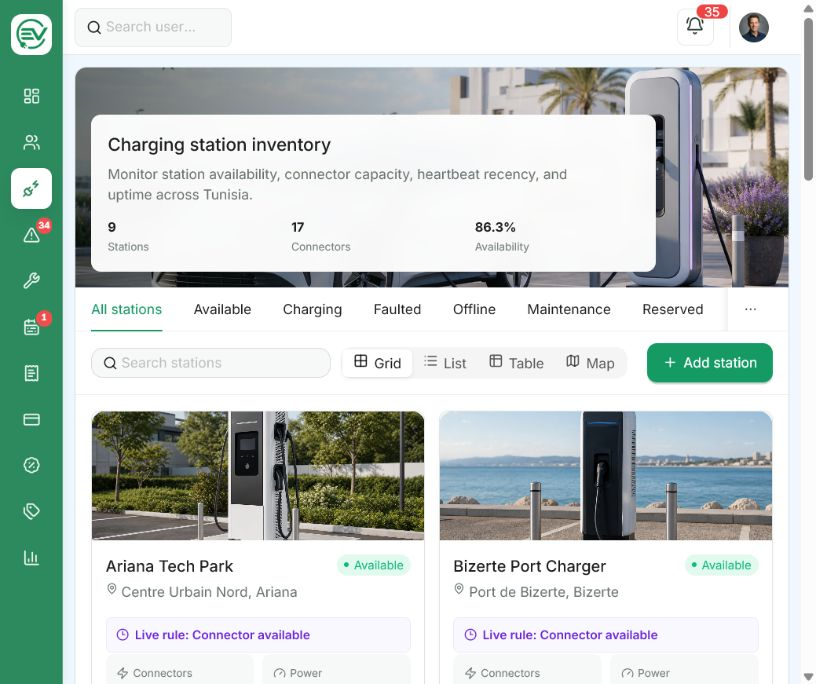
\includegraphics[width=0.93\textwidth]{assets/screenshots/stations-workspace.png}
  \caption{Inventaire des stations avec indicateurs de disponibilité}
  \label{fig:implementation-station-inventory}
\end{figure}

Leaflet et OpenStreetMap permettent de placer un marqueur par clic ou
glisser-déposer. Les coordonnées restent éditables pour traiter les cas où la
géolocalisation est imprécise. Côté client, la préférence de rayon
\emph{Near me} limite la recherche autour de la position autorisée par le
navigateur. Le frontend peut également copier les coordonnées ou ouvrir
l'itinéraire dans un service cartographique externe.

\subsubsection{Commissioning atomique}

La simple création d'une ligne en base ne suffit pas à rendre une borne
exploitable. Un assistant de commissioning regroupe l'identité de la station, son
matériel, ses connecteurs et son profil de simulateur. La référence interne et
l'identité OCPP sont contrôlées avant la transaction. Pour une cible locale, le
backend prépare un profil que le simulateur SAP peut enregistrer.

\begin{figure}[H]
  \centering
  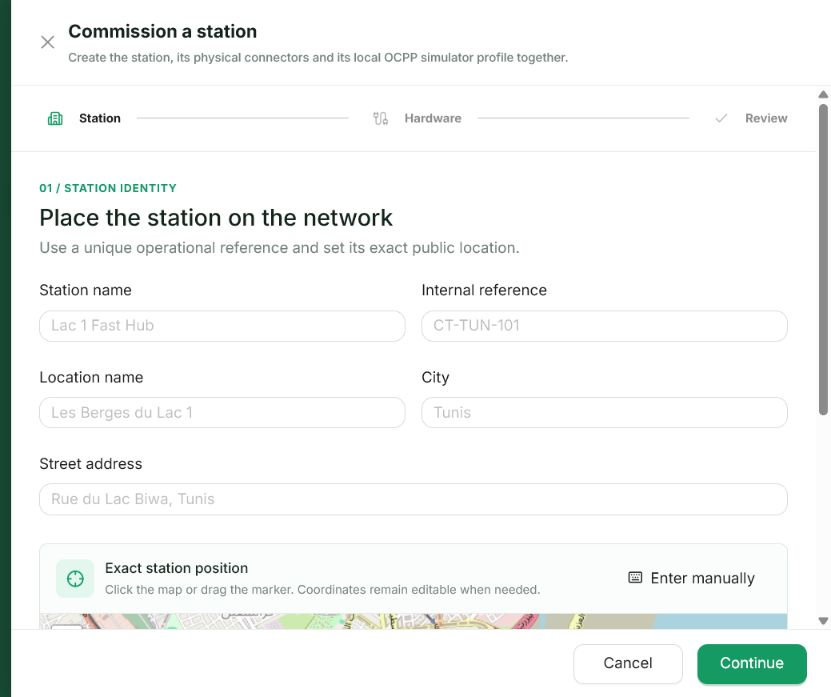
\includegraphics[width=0.93\textwidth]{assets/screenshots/station-commissioning.png}
  \caption{Première étape du commissioning guidé d'une station}
  \label{fig:implementation-station-commissioning}
\end{figure}

\texttt{StationCommissioningService} exécute la création de la station, des
connecteurs et des accès OCPP dans une transaction. Si une référence, une
identité ou un connecteur est invalide, aucune création partielle ne subsiste. Le
secret éventuel d'une borne physique n'est affiché qu'une fois et seul son
condensat est conservé.

Les QR codes sont dérivés d'un jeton de connecteur destiné au parcours client. Le
code affiché dans l'espace d'exploitation sert à imprimer l'étiquette physique ;
le client utilise ensuite le scanner pour identifier le connecteur sans saisir
manuellement sa référence. La plateforme ne considère toutefois pas le scan
comme une preuve suffisante : la disponibilité et le démarrage restent validés
par le backend et par OCPP.

Les documents de station sont persistés avec leur type, leur propriétaire et
leur périmètre. Les autorisations distinguent contrats, garanties, notices et
plans techniques. L'API ne retourne jamais un chemin arbitraire du système de
fichiers ; le téléchargement passe par un contrôleur autorisé.

\subsection{INC-03 : OCPP et disponibilité calculée}

\subsubsection{Connexion de la borne simulée}

La passerelle Python reçoit les connexions WebSocket OCPP 1.6 JSON. Au démarrage,
le simulateur envoie \texttt{BootNotification}, puis des
\texttt{Heartbeat} périodiques et des \texttt{StatusNotification} pour chaque
connecteur. La passerelle normalise le message et l'envoie à une API interne
Laravel signée. Elle ne calcule pas l'état métier et n'écrit pas dans PostgreSQL.

\texttt{OcppEventIngestionService} enregistre l'événement brut utile à l'audit,
met à jour les projections techniques et délègue les décisions à
\texttt{AvailabilityProjectionService} ou
\texttt{OcppTransactionProjectionService}. L'identifiant de la station présent
dans l'URL WebSocket doit correspondre exactement à l'identité provisionnée.

\begin{figure}[H]
  \centering
  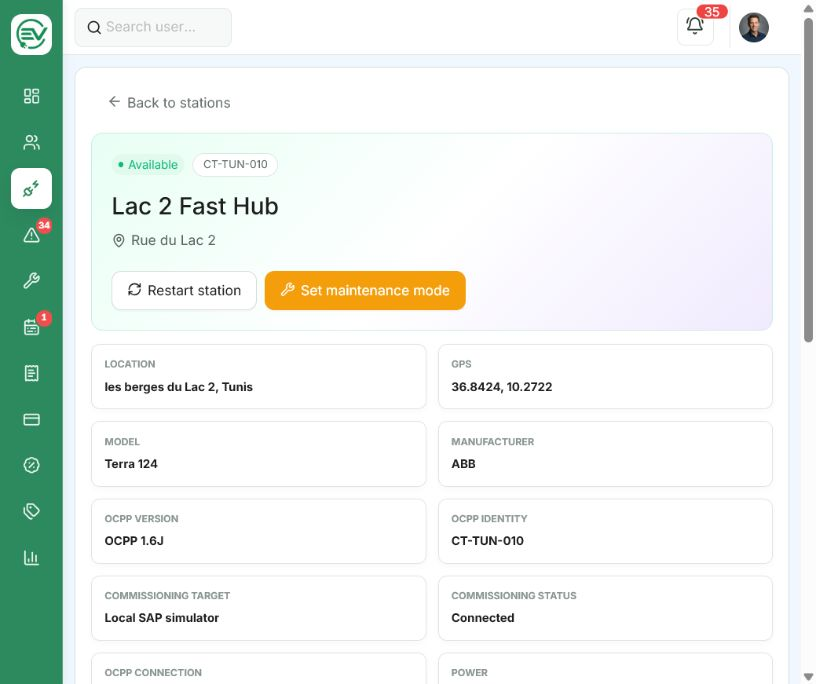
\includegraphics[width=0.88\textwidth]{assets/screenshots/station-detail.png}
  \caption{Fiche d'une station reliée au simulateur SAP}
  \label{fig:implementation-station-connected}
\end{figure}

\subsubsection{Règles de projection}

L'état affiché n'est pas un champ saisi manuellement. Il est reconstruit à partir
des preuves disponibles selon un ordre de priorité. Une maintenance active ou
une désactivation administrative peut rendre l'actif indisponible. Une absence
de signal au-delà du délai configuré produit l'état déconnecté. Un code d'erreur
OCPP actif produit l'état en défaut. Une transaction active rend le connecteur
occupé. En l'absence de ces conditions, le dernier
\texttt{StatusNotification} détermine notamment les états disponible, réservé ou
indisponible.

\begin{table}[H]
  \centering
  \caption{Exemples de règles de disponibilité réalisées}
  \label{tab:implementation-availability-rules}
  \begin{tabularx}{\textwidth}{@{}p{3.3cm}p{5.1cm}Y@{}}
    \toprule
    \textbf{État projeté} & \textbf{Preuve dominante} &
    \textbf{Conséquence}\\
    \midrule
    Disponible & Statut OCPP \texttt{Available}, signal récent et aucune
    contrainte prioritaire & Le connecteur peut être proposé au client.\\
    Occupé & Transaction OCPP active ou statut \texttt{Charging} &
    Le connecteur n'est plus sélectionnable pour une nouvelle session.\\
    Réservé & Statut \texttt{Reserved} ou réservation valide &
    L'accès est limité au bénéficiaire attendu.\\
    Maintenance & Fenêtre de maintenance active ou commande de changement de
    disponibilité & Le connecteur est retiré du service.\\
    En défaut & Code d'erreur ou statut \texttt{Faulted} &
    Une alerte opérationnelle est créée ou actualisée.\\
    Déconnecté & Aucun heartbeat ou événement dans le délai configuré &
    La station est indisponible et une alerte de communication est ouverte.\\
    \bottomrule
  \end{tabularx}
\end{table}

Le recalcul est idempotent : recevoir plusieurs fois la même preuve ne crée pas
une suite d'alertes identiques. Lorsque la communication revient, la projection
est réévaluée et l'alerte peut être résolue selon sa règle. Les transitions sont
horodatées afin de calculer l'uptime sur une période.

\subsubsection{Commandes et télémétrie}

Depuis la fiche station, un utilisateur autorisé peut demander
\texttt{Reset}, \texttt{UnlockConnector} ou
\texttt{ChangeAvailability}. Laravel crée d'abord une commande avec un état
attendu, puis la passerelle la récupère et transmet l'appel à la borne. La réponse
de la borne met à jour le résultat ; une tâche planifiée expire les commandes qui
ne reçoivent pas de réponse. Le bouton n'affirme donc jamais qu'une action
physique a réussi avant l'accusé OCPP.

\path{MeterValues} alimente la puissance et l'énergie réellement rapportées.
L'interface distingue ces mesures des statistiques calculées à partir des
sessions. Lorsqu'aucun \texttt{MeterValues} n'a été reçu, elle affiche
\emph{No signal} au lieu de générer une série visuelle artificielle.

\begin{figure}[H]
  \centering
  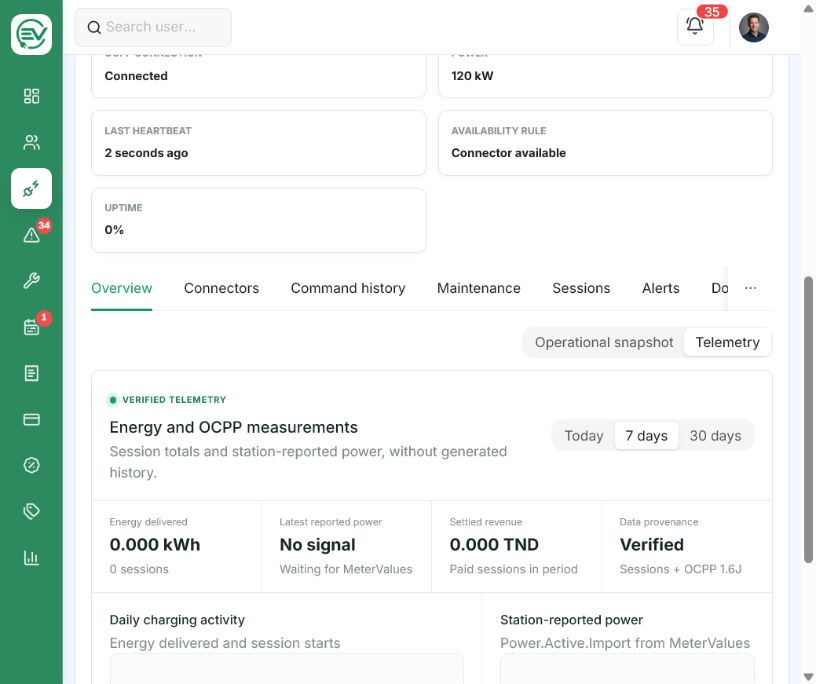
\includegraphics[width=0.88\textwidth]{assets/screenshots/station-telemetry.png}
  \caption{Télémétrie vérifiée sans génération de mesures fictives}
  \label{fig:implementation-station-telemetry}
\end{figure}

Les tests \path{OcppGatewayApiTest},
\path{OcppSimulatorFleetTest}, \path{OcppSupervisionApiTest},
\path{OcppTransactionProjectionTest},
\path{AvailabilityProjectionTest} et
\path{StationTelemetryApiTest} vérifient les contrats, la déduplication, les
transitions et l'isolation des organisations.

\section{Réalisation des parcours métier}

\subsection{Sprint 6 : exploitation terrain}

\subsubsection{Alertes et qualification}

Une alerte représente un symptôme opérationnel à traiter, et non une intervention.
Elle possède une sévérité, un statut, une station, un contexte technique et une
chronologie. Elle peut provenir automatiquement d'une perte de communication,
d'un défaut OCPP ou d'une règle de maintenance, mais un utilisateur autorisé peut
également créer une alerte manuelle.

L'interface utilise une disposition en deux panneaux : la liste filtrable reste
visible pendant que le détail, les actions et l'historique de l'alerte sélectionnée
sont consultés. Les filtres de sévérité et d'état ne modifient pas la donnée ; ils
sont convertis en paramètres API. Les compteurs de la barre latérale sont dérivés
des notifications non lues liées à ce contexte.

La figure~\ref{fig:interfaces-alerts} présente l'organisation visuelle de ce
centre opérationnel dans le chapitre suivant.

\subsubsection{Interventions, maintenance et SLA}

Une intervention matérialise le travail humain déclenché par une alerte ou une
décision d'exploitation. L'opérateur la crée, choisit une priorité et l'assigne à
un technicien de la même organisation. Le technicien accepte le travail, ajoute
ses notes, documente le diagnostic, les actions et les pièces, joint des photos
\emph{avant/après}, puis soumet son rapport. L'opérateur contrôle ensuite le
résultat et clôt l'intervention.

La maintenance répond à un besoin différent. Elle planifie une action préventive
ou corrective sur une période, indépendamment de l'existence immédiate d'une
alerte. \texttt{MaintenancePlanService} gère le plan, tandis que
\texttt{MaintenanceLifecycleService} contrôle les transitions. Le job
\texttt{GenerateMaintenanceOccurrences} matérialise les occurrences récurrentes.

\texttt{NotificationSlaService} analyse chaque minute les échéances approchantes
ou dépassées. Les notifications sont enregistrées en base, diffusées par Reverb
et éventuellement envoyées par email via la queue. L'utilisateur peut marquer
une notification lue globalement ou dans le contexte de la page consultée.

Les documents d'alerte, d'intervention et de maintenance sont générés par le
backend. Le rapport PDF reprend la référence, les acteurs, les dates, les preuves
et l'historique sans dépendre d'une capture de l'écran. Les pièces jointes passent
par des routes autorisées et sont supprimables selon le cycle de vie de la
ressource.

\subsection{Sprint 5 : recharge, transaction et paiement}

\subsubsection{Assistant de recharge client}

Le client peut ouvrir l'assistant depuis \emph{Start session}, depuis une fiche
station ou depuis la carte. Dans les deux derniers cas, la station est déjà
sélectionnée et le parcours commence directement au choix du connecteur. Le
workflow se compose de cinq étapes :

\begin{enumerate}[leftmargin=8mm]
  \item sélectionner une station disponible ;
  \item choisir un connecteur compatible et libre ;
  \item brancher le câble et attendre la confirmation OCPP ;
  \item autoriser le paiement simulé et vérifier le tarif applicable ;
  \item envoyer la demande de démarrage distant et attendre la transaction OCPP.
\end{enumerate}

Le passage de l'étape de branchement n'est pas manuel. Le frontend interroge la
tentative de recharge et reçoit la mise à jour du connecteur ; il avance uniquement
lorsque le backend confirme une preuve OCPP compatible. Les pictogrammes de prises
aident le client à reconnaître CCS2, Type~2, CHAdeMO ou un autre standard.

\subsubsection{Cycle de session}

\texttt{ChargingAttemptService} conserve le contexte entre les étapes et refuse
une station, un connecteur ou un tarif devenus invalides. Après autorisation,
\texttt{OcppCommandService} demande un
\texttt{RemoteStartTransaction}. Le simulateur répond, puis
\texttt{StartTransaction} devient la preuve de démarrage. Les
\texttt{MeterValues} actualisent l'énergie, la puissance et l'estimation. Le
client peut laisser la vue active en arrière-plan et y revenir depuis la page des
sessions.

\begin{figure}[H]
  \centering
  \begin{tikzpicture}[
    node distance=8mm and 7mm,
    workflowstep/.style={draw=ctline,fill=ctpaper,rounded corners=2mm,
      minimum width=2.65cm,minimum height=1.05cm,align=center,
      font=\small\bfseries,text=ctdark},
    flow/.style={-{Latex[length=2mm]},thick,draw=ctgreen}
  ]
    \node[workflowstep] (select) {Station et\\connecteur};
    \node[workflowstep,right=of select] (plug) {Branchement\\confirmé OCPP};
    \node[workflowstep,right=of plug] (auth) {Autorisation\\de paiement};
    \node[workflowstep,below=of auth] (start) {Transaction\\démarrée};
    \node[workflowstep,left=of start] (meter) {Mesures et\\estimation};
    \node[workflowstep,left=of meter] (stop) {Arrêt, capture\\et reçu};
    \draw[flow] (select) -- (plug);
    \draw[flow] (plug) -- (auth);
    \draw[flow] (auth) -- (start);
    \draw[flow] (start) -- (meter);
    \draw[flow] (meter) -- (stop);
  \end{tikzpicture}
  \caption{Parcours vertical d'une recharge}
  \label{fig:implementation-charging-flow}
\end{figure}

L'arrêt peut être demandé par le client, par un opérateur autorisé, par la borne
ou par une condition technique. \texttt{StopTransaction} clôt la transaction et
fige les valeurs finales. Le coût n'est pas calculé dans React :
\texttt{TariffResolver} sélectionne la règle applicable, puis le backend calcule
les composantes énergie, temps, forfait et remise.

\subsubsection{Adaptateur de paiement simulé}

Le domaine dépend de l'interface \path{PaymentGateway}. Deux implémentations sont
disponibles : \path{SimulatedPaymentAdapter}, utile aux tests unitaires, et
\path{WireMockPaymentAdapter}, qui appelle un serveur HTTP externe local. Les
opérations fonctionnelles sont l'autorisation, la capture, la libération et le
débit direct.

WireMock reproduit des succès, refus, délais, erreurs serveur et webhooks. Le
webhook est signé ; \path{PaymentWebhookSignature} vérifie son authenticité et
\path{PaymentProviderEventService} assure l'idempotence. Un même événement
rejoué ne capture donc pas deux fois une session. Le reçu est consultable dans
l'application et exportable en PDF.

Ce choix ne simule pas une banque au niveau réglementaire. Il valide la frontière
technique qui permettra d'ajouter ultérieurement ClicToPay, e-DINAR/D17,
GPGCheckout, Konnect ou Flouci. L'adaptateur réel devra ajouter la conformité du
prestataire, le rapprochement, la gestion des litiges et des remboursements.

\subsection{Sprint 7 : tarification et commerce}

\subsubsection{Tarifs et plans de recharge}

Un tarif appartient à une organisation et peut combiner un prix au kWh, un prix
au temps, un coût fixe et des règles horaires. Les affectations définissent son
périmètre : organisation, station ou connecteur. Lorsqu'une session commence,
\texttt{TariffResolver} applique l'affectation la plus spécifique et conserve une
référence au tarif retenu afin qu'une modification future ne change pas
rétroactivement le calcul.

Les plans clients sont des avantages proposés par une organisation : remise sur
la recharge, éventuel abonnement périodique et conditions d'accès. Un client peut
cumuler des abonnements auprès de plusieurs réseaux, car son utilisation d'une
borne ne le transforme pas automatiquement en client exclusif de son propriétaire.
La simple recharge crée une relation transactionnelle ; l'abonnement demeure une
décision explicite.

\subsubsection{Abonnement SaaS de l'organisation}

Le contrat commercial de l'organisation est volontairement séparé des paiements
des conducteurs. Il détermine la période d'essai, le nombre maximal d'employés et
de stations, les fonctions accessibles, la date de renouvellement et les factures
adressées à l'organisation. \texttt{OrganizationEntitlementService} contrôle les
limites avant la création d'un actif, tandis que
\texttt{OrganizationSubscriptionLifecycleService} traite essai, activation,
suspension, expiration et restauration.

L'interface de suivi de l'abonnement est reproduite dans la
figure~\ref{fig:interfaces-organization-billing}.

Le super administrateur gère le catalogue SaaS et le portefeuille global.
L'administrateur consulte son offre, sa consommation de capacité et ses factures,
puis émet une demande de changement. Cette demande évite qu'un administrateur
modifie directement un contrat financier. L'encaissement SaaS reste simulé ou
manuel dans le MVP.

\subsection{Sprint 8 : pilotage, reporting et gouvernance}

\subsubsection{Tableaux de bord par rôle}

\texttt{DashboardService} compose une réponse différente selon le rôle plutôt que
de renvoyer le même tableau de bord avec des libellés modifiés. Le super
administrateur supervise les organisations et les intégrations. L'administrateur
observe les employés, clients, revenus, stations et performances de son
organisation. L'opérateur suit disponibilité, incidents et sessions. Le
technicien voit sa charge terrain et ses SLA. Le client consulte ses recharges,
paiements et abonnements.

La figure~\ref{fig:interfaces-admin-dashboard} montre la composition retenue
pour le tableau de bord de l'administrateur.

Les indicateurs utilisent les mêmes règles et périmètres que les écrans de détail.
Par exemple, la disponibilité du tableau de bord passe par
\texttt{AvailabilityMetrics} et ne moyenne pas des valeurs fictives du frontend.
Les sélecteurs de période sont transformés en bornes temporelles côté API.

\subsubsection{Rapports et échanges internes}

Les espaces d'analyse sont adaptés au périmètre du rôle :
\texttt{/reporting/platform}, \texttt{/organization},
\texttt{/operations} et \texttt{/field}. Les exports PDF, JSON et CSV réutilisent
les mêmes filtres et autorisations. Les rapports internes sont des objets
distincts des exports : un employé peut composer un rapport, joindre des fichiers,
choisir un destinataire de son organisation, l'envoyer, puis suivre lecture et
archivage.

La figure~\ref{fig:interfaces-admin-reports} illustre cet espace d'analyse et
d'échange.

\subsubsection{Administration globale}

Le super administrateur dispose d'un espace cohérent avec la navigation du
produit, mais orienté opérations de plateforme : organisations, utilisateurs,
rôles, permissions, demandes de démonstration, catalogue commercial, audit,
intégrations et paramètres. Les secrets OAuth, OCPP, email ou paiement ne sont
jamais renvoyés par les endpoints d'intégration. L'écran expose uniquement l'état
de configuration et la date du dernier contrôle.

\texttt{PlatformSettingService} limite les paramètres modifiables à une liste
validée. Les valeurs sensibles restent dans l'environnement. Toute modification
globale est attribuée à son auteur dans le journal d'audit. Les paramètres
personnels, tels que fuseau horaire, préférences de notification et rayon de
recherche, restent séparés des contrôles globaux.

\subsection{Sprint 9 : exports et évolutions différées}

\texttt{ReportExportService} centralise les formats PDF, CSV et JSON. OpenSpout est
disponible pour les formats tabulaires plus riches, tandis que DomPDF produit les
documents visuels. Les reçus, factures et rapports opérationnels sont générés près
de leur ressource afin que l'utilisateur les retrouve dans le workflow concerné,
et non uniquement dans une page de rapports générique.

La gestion distante du firmware n'est pas simulée comme si elle était achevée.
Elle nécessite une matrice de compatibilité matériel/logiciel, la signature des
paquets, un hébergement sécurisé, le suivi de progression, une stratégie de
retour arrière et une validation sur borne. Elle reste donc une évolution du
Product Backlog non engagée dans le MVP, conformément au risque de 13 points
associé à US-38.

\section{Tests et débogage}

\subsection{Stratégie de tests}

La stratégie accorde la priorité aux invariants backend, car le frontend ne doit
pas être la seule barrière contre une action interdite. La campagne principale
utilise SQLite en mémoire, une queue synchrone, un mailer en mémoire et un
diffuseur nul afin de rester rapide et reproductible. Un second ensemble est
exécuté avec PostgreSQL et Redis dans GitHub Actions afin de vérifier les
migrations, les requêtes spécifiques au moteur et l'infrastructure réellement
utilisée en production. Aucun email réel ni événement WebSocket public n'est
émis pendant ces campagnes.

\begin{longtable}{|p{2.8cm}|p{3.9cm}|p{3.9cm}|p{2.8cm}|}
  \caption{Niveaux de validation appliqués}
  \label{tab:implementation-test-strategy}\\
  \hline
  \textbf{Niveau} & \textbf{Objet} & \textbf{Exemples} &
  \textbf{Preuve}\\
  \hline
  \endfirsthead
  \hline
  \textbf{Niveau} & \textbf{Objet} & \textbf{Exemples} &
  \textbf{Preuve}\\
  \hline
  \endhead
  Tests métier & Invariants, projections et transitions &
  disponibilité, transactions OCPP, tarifs, cycles commerciaux &
  Assertions PHPUnit.\\\hline
  Tests API & Validation, autorisation, sérialisation et effets &
  authentification, stations, alertes, rapports, paiement &
  Réponses et base vérifiées.\\\hline
  Tests d'isolation & Accès croisé entre organisations &
  utilisateurs, actifs, interventions, exports &
  Réponses 403/404 attendues.\\\hline
  Tests d'adaptateur & Contrat avec un service remplaçable &
  WireMock, webhook signé, Google OAuth simulé &
  Doubles et serveur local.\\\hline
  Tests OCPP & Lecture des profils et scénarios du simulateur &
  connexion, plug/unplug, transactions, projections &
  Node Test et PHPUnit.\\\hline
  Qualité frontend & Types, imports et règles statiques &
  compilation Vite et Oxlint &
  Commandes sans erreur.\\\hline
  Vérification visuelle & Mise en page et parcours représentatifs &
  dashboards, stations, cartes, formulaires, documents &
  Inspection navigateur/PDF.\\
  \hline
\end{longtable}

\subsection{Résultats mesurés}

La campagne d'intégration continue exécutée le 13 août 2026 produit les résultats
suivants :

\begin{table}[H]
  \centering
  \caption{Résultats de validation du dépôt}
  \label{tab:implementation-test-results}
  \begin{tabularx}{\textwidth}{|p{4.5cm}|p{3.2cm}|Y|}
    \hline
    \rowcolor{ctmint}
    \textbf{Contrôle} & \textbf{Résultat} & \textbf{Portée}\\\hline

    Tests backend complets &
    265 tests, 2\,761 assertions & Tests Feature et unitaires chargés par
    PHPUnit avec SQLite.\\\hline
    Compatibilité PostgreSQL &
    20 tests, 153 assertions & Migrations, requêtes et contraintes exécutées
    avec PostgreSQL~18.\\\hline
    \texttt{python -m pytest} dans \texttt{ocpp-gateway} &
    23 tests, 0 échec & Messages entrants, commandes distantes, signatures et
    identifiants d'événements.\\\hline
    Tests frontend &
    39 tests, 0 échec & Composants, contrats, utilitaires et comportements
    critiques, complétés par Oxlint et la compilation Vite.\\\hline
    Tests infrastructure et outils &
    39 tests, 0 échec & Compose, CI/CD, sauvegarde, politiques de secrets,
    Simulation Lab et outils OCPP.\\\hline
    Construction Docker &
    Succès & Images de l'API, du frontend, de la passerelle et des simulateurs.\\\hline

  \end{tabularx}
\end{table}

La réussite de la compilation ne prouve pas seule la qualité UX, et le nombre de
tests ne remplace pas une recette. Elle montre néanmoins que les contrats
principaux, les migrations et la majorité des cycles de vie restent cohérents
après l'intégration des développements successifs.

\subsection{Anomalies représentatives et non-régression}

Plusieurs anomalies rencontrées pendant la réalisation ont renforcé les contrôles :

\begin{itemize}[leftmargin=7mm]
  \item une requête depuis l'adresse locale du réseau pouvait recevoir une erreur
  419 lorsque les domaines de session et les origines CSRF ne couvraient que
  \texttt{localhost}. La configuration a été rendue cohérente pour l'hôte local et
  l'adresse LAN de développement ;
  \item une double soumission involontaire d'une invitation déclenchait une erreur
  429. Le bouton est verrouillé pendant la requête et les limites restent actives
  côté serveur ;
  \item un tri \texttt{created\_at} combiné à un \texttt{GROUP BY} était accepté
  par certains moteurs mais refusé par PostgreSQL. La requête d'agrégation des
  photos d'intervention a été corrigée et couverte par un test ;
  \item \texttt{crypto.randomUUID()} échouait sur un navigateur mobile servi en
  HTTP non sécurisé. L'identifiant temporaire utilise désormais une solution
  compatible qui ne modifie pas l'identité métier du backend ;
  \item des URL WebSocket figées sur \texttt{localhost} empêchaient Reverb de
  fonctionner depuis un téléphone. Le frontend construit l'hôte de développement
  à partir de sa configuration plutôt que de supposer une machine unique.
\end{itemize}

Les réponses d'erreur de l'API sont normalisées pour ne pas exposer une trace SQL,
un chemin local ou un secret. En environnement de production,
\texttt{APP\_DEBUG=false} reste obligatoire.

\section{Intégration des composants}

\subsection{Intégration bout en bout}

L'intégration verticale est vérifiable sans accès direct du frontend à la borne
ou au fournisseur de paiement. React appelle uniquement l'API publique Laravel.
Laravel crée les intentions métier et les commandes. La passerelle OCPP échange
avec le simulateur puis renvoie des événements signés. PostgreSQL conserve les
preuves et projections. Reverb diffuse les changements utiles à l'interface.
WireMock représente un système financier externe indépendant.

\begin{figure}[H]
  \centering
  \begin{tikzpicture}[
    node distance=7mm and 8mm,
    box/.style={draw=ctline,fill=ctpaper,rounded corners=2mm,
      minimum width=2.7cm,minimum height=1.0cm,align=center,
      font=\small\bfseries,text=ctdark},
    arrow/.style={-{Latex[length=2mm]},thick,draw=ctgreen}
  ]
    \node[box] (react) {React};
    \node[box,right=of react] (laravel) {Laravel};
    \node[box,right=of laravel] (db) {PostgreSQL};
    \node[box,below=of laravel] (gateway) {Passerelle OCPP};
    \node[box,left=of gateway] (simulator) {Simulateur SAP};
    \node[box,right=of gateway] (payment) {WireMock};
    \draw[arrow] (react) -- node[above,font=\scriptsize]{HTTP} (laravel);
    \draw[arrow] (laravel) -- node[above,font=\scriptsize]{transactions} (db);
    \draw[arrow] (laravel) -- node[right,font=\scriptsize]{commandes} (gateway);
    \draw[arrow] (gateway) -- node[below,font=\scriptsize]{WebSocket OCPP} (simulator);
    \draw[arrow] (laravel) -- node[above right,font=\scriptsize]{paiement} (payment);
    \draw[arrow,dashed] (laravel) to[bend left=20]
      node[above,font=\scriptsize]{Reverb} (react);
  \end{tikzpicture}
  \caption{Composants traversés par le MVP vertical}
  \label{fig:implementation-vertical-integration}
\end{figure}

Cette structure facilite le diagnostic. Un écran n'actualisant pas une donnée
peut être analysé successivement au niveau de la requête React, de la réponse API,
de la projection PostgreSQL, de l'événement reçu par la passerelle et du message
émis par le simulateur.

\subsection{Services externes intégrés}

\begin{table}[H]
  \centering
  \caption{Intégrations techniques et responsabilités}
  \label{tab:external-integrations}
  \begin{tabularx}{\textwidth}{|p{3.0cm}|p{3.1cm}|Y|Y|}
    \hline
    \rowcolor{ctmint}
    \textbf{Intégration} & \textbf{Technologie} & \textbf{Responsabilité} &
    \textbf{Frontière}\\\hline
    Identité sociale & Google OAuth 2.0 & Vérifier l'identité et l'email &
    Les rôles et organisations restent locaux.\\\hline
    Email transactionnel & Resend & Envoyer vérifications, invitations et alertes &
    Les secrets et l'envoi restent côté serveur.\\\hline
    Cartographie & Leaflet / OpenStreetMap & Afficher tuiles, marqueurs et itinéraires &
    La position courante du client n'est pas persistée.\\\hline
    Paiement & Adaptateur de paiement & Autoriser, capturer, libérer ou débiter &
    Le fournisseur ne modifie jamais directement une session.\\\hline
    Simulation du paiement & WireMock 3 & Reproduire succès, refus, délai et webhook &
    Aucun moyen de paiement réel n'est utilisé.\\\hline
    Simulation des bornes & Simulateur SAP & Produire des connexions et messages OCPP &
    Le simulateur ne lit ni l'API métier ni la base.\\\hline
  \end{tabularx}
\end{table}

\section{Validation et vérification}

\subsection{Limites de la validation}

\begin{scopebox}[Frontière des résultats]
\begin{itemize}[leftmargin=7mm]
  \item Le simulateur SAP valide les messages OCPP 1.6J, mais pas le comportement
  électrique, le modem ou le firmware d'une borne réelle.
  \item WireMock valide le contrat HTTP et les webhooks, mais aucune transaction
  bancaire ni exigence PCI DSS.
  \item Les tests automatisés n'ont pas encore été complétés par une campagne de
  charge OCPP multi-borne ni par des tests de performance formels.
  \item Le déploiement public, TLS, CI/CD et les sauvegardes sont opérationnels,
  mais ils n'ont pas encore fait l'objet d'une mesure de disponibilité de longue
  durée, d'un test de charge représentatif ni d'un exercice complet de reprise.
  \item La recette fonctionnelle formelle et son procès-verbal restent à réaliser
  avec le représentant habilité de l'entreprise.
  \item OCPP 2.0.1, Microsoft OAuth, le paiement réel et le firmware restent hors
  du MVP validé.
\end{itemize}
\end{scopebox}

\subsection{Évolution par rapport au cahier des charges initial}
\label{subsec:scope-evolution}

Le \emph{Cahier des Charges Fonctionnel -- Développement d'une plateforme Web
de Gestion des Bornes de Recharge Électrique Connectées}, version 1.0, constitue
la référence initiale transmise par l'entreprise \cite{tacticCahierCharges2026}.
Il décrit un produit cible large et conserve volontairement plusieurs
alternatives technologiques. Le Product Backlog et les revues de Sprint ont
transformé cette intention en un MVP vérifiable sans modifier rétroactivement
le document d'origine.

\begin{longtable}{|p{3.0cm}|p{4.5cm}|p{6.8cm}|}
  \caption{Principales adaptations du périmètre initial}
  \label{tab:scope-main-adaptations}\\
  \hline
  \textbf{Décision} & \textbf{Prévision initiale} & \textbf{Choix retenu et justification}\\
  \hline
  \endfirsthead
  \hline
  \textbf{Décision} & \textbf{Prévision initiale} & \textbf{Choix retenu et justification}\\
  \hline
  \endhead
  Socle backend & Laravel 12, PHP 8.3 et JWT &
  Laravel 13 sur PHP 8.5 local, avec compatibilité Composer à partir de PHP 8.3.
  Sanctum protège la SPA par session et CSRF, sans jeton JWT stocké dans le
  navigateur.\\\hline
  Traitements internes & Redis pour cache et files &
  Redis~7 est utilisé pour le cache, les sessions et les files d'attente, tandis
  que PostgreSQL reste réservé aux données métier persistantes.\\\hline
  Interface analytique & React, Ant Design, TypeScript et ECharts &
  React, Ant Design et TypeScript sont conservés ; Recharts remplace ECharts
  dans les tableaux de bord, sans changer les besoins métier.\\\hline
  Protocole de borne & OCPP 1.6 et OCPP 2.0.1 &
  OCPP 1.6J est implémenté et testé avec la passerelle et le simulateur SAP.
  OCPP 2.0.1 est reporté afin de stabiliser d'abord le parcours vertical.\\\hline
  Paiement & Carte, portefeuille, paiement différé et remboursement &
  Un contrat de paiement remplaçable est validé avec WireMock et des méthodes
  carte, e-DINAR et D17 simulées. Aucun débit bancaire ni remboursement réel
  n'est revendiqué.\\\hline
  Équipement physique & Réseau de bornes connectées &
  Le commissioning, l'authentification et les échanges sont démontrés avec un
  simulateur OCPP. La validation électrique, modem et firmware exige une borne
  physique distincte.\\\hline
  Modules différés & Véhicules, RFID complet et firmware &
  L'identifiant OCPP virtuel et le QR d'entrée couvrent le démarrage du MVP.
  Les profils véhicule, les badges RFID physiques et la gestion distante du
  firmware sont exclus de la version validée.\\
  \hline
\end{longtable}

La matrice détaillée de l'annexe~\ref{app:specification-coverage} reprend les
18 modules, les messages OCPP, les choix d'architecture, les exigences non
fonctionnelles, les interfaces et les livrables. Elle emploie cinq statuts :
\emph{réalisée}, \emph{adaptée}, \emph{partielle}, \emph{reportée} et
\emph{à valider en production}. Neuf modules sont réalisés ou adaptés au MVP,
sept sont partiels et deux sont reportés. Cette lecture distingue ainsi un
écart assumé d'une fonctionnalité simplement oubliée.

\subsection{Traçabilité avec le backlog et les Sprints}

\begin{longtable}{|C{1.5cm}|p{3.3cm}|p{4.5cm}|p{4.0cm}|}
  \caption{Preuves de réalisation par Sprint}
  \label{tab:implementation-traceability}\\
  \hline
  \textbf{Sprint} & \textbf{User stories} & \textbf{Preuves dans le code} &
  \textbf{Tests principaux}\\
  \hline
  \endfirsthead
  \hline
  \textbf{Sprint} & \textbf{User stories} & \textbf{Preuves dans le code} &
  \textbf{Tests principaux}\\
  \hline
  \endhead
  S01 & US-27, 39 et travaux de conception &
  Backlog, cas d'utilisation global, architecture et prototype &
  Relectures, validation des parcours et démonstration du prototype.\\\hline
  S02 & US-01--04, 06 &
  Auth, Google, invitations, démo, onboarding, policies &
  Auth, OAuth, onboarding, utilisateurs, organisations.\\\hline
  S03 & US-07--13, 37 &
  Stations, connecteurs, cartes, commissioning, documents &
  Station API, commissioning, documents.\\\hline
  S04 & US-14--16, 19 &
  Gateway, ingestion, projection, commandes, télémétrie &
  OCPP gateway, flotte, supervision, disponibilité, télémétrie.\\\hline
  S05 & US-24--26, 28--30 &
  Tentatives, sessions, transactions, paiements, reçus &
  Recharge distante, session/paiement, webhook WireMock.\\\hline
  S06 & US-20--23, 40 &
  Alertes, interventions, maintenance, SLA, notifications &
  Alertes, rapports terrain, maintenance, notifications.\\\hline
  S07 & US-31, 32, 41, 42 &
  Tarifs, plans, abonnements clients et SaaS &
  Tarifs, plans, commercial organisationnel.\\\hline
  S08 & US-05, 17, 18, 33--36 &
  Dashboards, reporting, audit, paramètres, intégrations &
  Dashboard, rapports, gouvernance, recherche.\\\hline
  S09 & Stabilisation et livrables &
  Exports, documentation, cahier de tests et préparation de la recette &
  Compilation, contrôles transversaux et validation des documents.\\\hline
  S10 & Industrialisation et démonstration publique &
  Docker unifié, Simulation Lab, Redis, CI/CD, Azure, domaine et sauvegardes &
  Tests de politique, construction des images, déploiement et contrôles de santé.\\
  \hline
\end{longtable}

\section{Optimisation des performances}

Les listes volumineuses utilisent pagination et filtres côté serveur. Les
relations nécessaires aux ressources API sont chargées explicitement afin de
limiter les requêtes répétitives. Les agrégats de tableaux de bord sont calculés
par période et périmètre plutôt que reconstruits dans le navigateur. Les travaux
lents, notamment les emails et certaines notifications, passent par la queue.

Pour OCPP, la passerelle conserve la connexion WebSocket mais délègue rapidement
l'événement à Laravel. Le recalcul de disponibilité est idempotent et protégé
contre le chevauchement. Les événements et mesures restent horodatés, ce qui
permet d'appliquer un délai de non-réponse sans dépendre de l'heure du navigateur.

Le frontend applique un découpage par route et charge à la demande les fonctions
coûteuses, notamment la visualisation PDF et le scanner QR. La compilation de
production est contrôlée par la CI. Une campagne Lighthouse sur réseau mobile,
des budgets de bundle et un test de charge multi-stations restent cependant à
formaliser avant de fixer des objectifs de performance contractuels.

\section{Documentation technique}

Le dépôt contient les scripts d'installation, les configurations d'exemple, les
procédures de déploiement et de sauvegarde, les commandes d'exploitation des
simulateurs et le présent rapport. Scramble génère
une spécification OpenAPI 3.1 versionnée dans
\path{docs/api/openapi.json} et une interface d'exploration protégée sous
\path{/docs/api}. Les routes internes OCPP et paiement restent volontairement
exclues de cette documentation publique.

Le manuel utilisateur, le manuel administrateur et le cahier de tests sont
également compilés et versionnés. Le procès-verbal de recette ne sera préparé
qu'au moment de la campagne fonctionnelle avec l'entreprise, puisqu'il devra
reprendre les résultats réellement observés, les réserves et la décision du
responsable habilité.


\section*{Conclusion}

La réalisation confirme la faisabilité de l'architecture proposée. Le dépôt
contient une application React par rôle, une API Laravel protégée, un modèle
PostgreSQL couvrant les domaines principaux, une passerelle OCPP indépendante et
des adaptateurs pour les services externes. Le simulateur SAP produit des
messages OCPP effectivement ingérés ; les services Laravel calculent ensuite les
projections de disponibilité, les sessions, les alertes et les données de
pilotage. Le paiement externe reste simulé, mais son contrat permet de remplacer
WireMock sans réécrire le parcours de recharge.

La campagne locale atteint 201 tests backend et 1\,489 assertions, complétés par
deux tests des outils OCPP, le lint frontend et une compilation de production.
Ces résultats valident le MVP vertical dans l'environnement du stage. Les
travaux encore ouverts concernent principalement l'industrialisation, la mesure
de charge, la documentation OpenAPI, la recette formelle, la connexion à un
prestataire financier réel, l'essai sur une borne physique et la gestion
sécurisée du firmware.
